\documentclass{article}
\usepackage{amsmath}
\usepackage{amssymb}
\usepackage{hyperref}
\usepackage{caption}
\usepackage{mathtools}
\usepackage{graphicx}
\usepackage{todonotes}
\graphicspath{{./images}}

\begin{document}

\title{Appunti molto belli di Algebra}
\author{Floppy Loppy}
\date{September 2021}
\maketitle
\tableofcontents
\newpage
\listoftodos\




\newpage
\section{Insiemi}
Noi definiamo \textbf{insieme} una \textbf{collezione} di elementi, questi elementi possono qualsiasi cosa: numeri, oggetti, persone, ecc.. \par
Gli elementi fanno parte di un insieme soltanto se rispettano le proprietà dell'insieme stesso, per esempio gli elementi dell'insieme dei numeri pari dovranno avere come proprietà quella di essere pari appunto. \par
Perfetto ora che abbiamo una definizione di insieme possiamo iniziare ad introdurre la sintassi e alcune proprietà.

\subsection{Proprietà degli insiemi}
Consideriamo di avere un insieme di nome \textit{A} e un elemento che chiamiamo \textit{x} che fa parte di \textit{A} (perchè rispetta le proprietà dell'insieme), allora si dice che \textit{x} \textbf{Appartiene} ad \textit{A}, ciò in Algebra si scrive:
\begin{equation}
        x \in A
\end{equation}

Mentre l'opposto ovvero che un elemento \textit{x} non fa parte di \textit{A} (perchè non rispetta le proprietà dell'insieme), allora si dice \textit{x} \textbf{Non Appartiene} ad \textit{A}, e ciò in si scrive (Nella lingua degli algebristi):
\begin{equation}
        x \not \in A
\end{equation}

Se un insieme ha più di un elemento, che possono essere \{\textit{x1,x2,\ldots,$x_n$}\} allora possiamo sintetizzare la scrittura del fatto che ognuno di questi elementi appartiene all'insieme \textit{A} scrivendo:
\begin{equation}
        x = \{x1,x2,\ldots,x_n\} 
\end{equation}

Oppure (visto che piace ai matematici) sintetizzare ancora di più scrivendo:
\begin{equation}
        A = \{x : P(x)\}
\end{equation}

Che si legge \textit{A uguale agli elementi di x tali che $P(x)$}, dove:
\begin{itemize}
        \item x sono gli elementi.
        \item $P(x)$ la proprietà dell'insieme \textit{A} che gli elementi di \textit{A} devono rispettare.
\end{itemize}
La proprietà $P(x)$ ha l'obbligo di essere \textbf{oggettiva} ovvero in grado di dare un valore oggettivamente vero o falso ad un elemento. \par
Possiamo utilizzare un esempio più concreto come può essere quello dei numeri pari scriviendo:
\begin{equation}
        A = \{x : x \quad \textrm{è un numero pari} \} 
\end{equation}

In questo caso possiamo dire che:
\begin{align*}
        2 \in A \\
        3 \not \in A \\
        Alessio \not \in A \\ 
\end{align*}
In quanto 2 è pari perciò appartiene ad A, 3 è dispari quindi non appartiene all'insieme e Alessio non è un numero pari quindi non può appartenere all'insieme descritto.

Questo perchè la proprietà di essere pari è \textbf{oggettiva} mentre per esempio:
\begin{equation}
        B = \{x : x \quad \textrm{è un libro interessante} \} 
\end{equation}
Non può essere un insieme in quanto essere un \textit{libro interessante} non è una proprietà oggettiva.

Proseguendo possiamo trovare anche insiemi che contengono un solo elemento, questi insiemi sono detti \textbf{singoletti} e sono scritti:
\begin{equation}\label{def_singoletto}
        \{*\}
\end{equation}
Dove * rappresenta il singolo elemento.

Ed infine, l'insieme vuoto che si rappresente con il simbolo:
\begin{equation}
        \emptyset 
\end{equation}
Spiegandolo brevemente questo insieme non contiene nessun elemento (infatti si definisce vuoto), e possiede alcune proprietà interessanti come per esempio quello di essere contenuto in qualsiasi insieme.


\subsection{Connettivi Logici}
Attraverso quelli che chiamiamo \textbf{connettivi logici} possiamo eseguire delle operazioni tra insiemi, da queste operazioni noi possiamo ricavare due valori: vero o falso,  andiamone a vederne alcune. \par

Prima di tutto definiamo due \textbf{proposizioni/affermazioni} fittizzie che chiamiamo $P$ e $D$ e partendo da questi andiamo a scrivere le operazioi che si possono effettuare su di essi:
\begin{itemize}
        \item La \textbf{Disgiunzione} scritta: $P \vee D$ ha valore vero quando almeno una delle due proposizione risulta vera, se entrambe sono false avremo invece un valore falso. 
        \item La \textbf{Congiunzione} scritta: $P \wedge D$ ha valore vero solo quando entrambe sono vere altrimenti otteniamo un valore falso.
        \item La \textbf{Negazione} scritta: $\lnot P$ inverte il valore della propsizione, se infatti P è vera $\lnot P$ sarà falsa e viceversa.
        \item L' \textbf{Implicazione} scritta: $P \Rightarrow D$ ha valore vero solo quando D è vera.
        \item L' \textbf{Equivalenza} scritta: $P \Leftrightarrow D$ ha valore vero solo quando P e D hanno lo stesso valore logico (vero;vero), (falso;falso).
\end{itemize}


\subsection{Quantificatori universali}
Abbiamo poi quelli che si chiamano quantificatori universali che servono a descrivere le proposizioni e le andremo a spiegare partendo da una proposizione qualsiasi che chiameremo $P$. \newline

Scriviamo:
\begin{equation}
P : \forall x \in A  
\end{equation}
per dire che \textbf{per ogni} elemento di $A$ la proposizione $P$ vale. \newline

Mentre scriviamo:
\begin{equation}
P : \exists x \in A  
\end{equation}
Per dire che \textbf{esiste almeno} un elemento di $A$ tale per cui la proposizione $P$ è vera. \\

Possiamo fare un esempio concreto, prendiamo un insieme $A = \{2,4,6,8\}$ e $P(x) = \textrm{x + 2 è pari}$ da questo possiamo dire con certezza che: 
\begin{align}
        \forall x \in A \quad P(x) \quad \textrm{è vera in quanto ogni elemento di A è pari} \\
        \exists x \in A \quad P(x) \quad \textrm{è vera in quanto almeno un elemento di A è pari}
\end{align}
\\

Abbiamo poi \textbf{l'esiste unico} che sta ad indicare che esiste un solo elemento in un dato insieme affinché una proposizione risulti vera:
\begin{equation}
        \exists! x \in A
\end{equation}


\subsection{Ordine dei quantificatori}
Come ogni cosa in matematica bisogna rispettare gli ordini delle varie operazioni e questo vale anche per i quantificatori universali, si abbia per esempio:
\begin{align}
        P: x+y = 0  \quad \mbox{allora:} \\
        \exists y \forall x P : \exists y \forall x \quad x + y = 0
\end{align}
La proposizione dice che esiste un numero che è opposto di ogni numero (perchè appunto un numero sommato al suo opposto è a zero). \par
Se cambiamo l'ordine dei quantificatori però cambiamo il significato di della proposizione, proviamo:
\begin{itemize}
        \item $\forall y \exists x P$ che significa che ogni y esiste almeno un opposto 	
        \item $\exists x \forall y$ che significa esiste almeno un x che è opposto a tutti i numeri
\end{itemize}
Come abbiamo visto abbiamo radicalmente cambiato il significato della proposizione P. \newline

Nel caso ci fossero ancora dubbi utilizzerò questo esempio: \newline
Prendiamo una proposizione $P$ che dice che x paga da bere a y, utilizzando gli esempi di prima avremo che:
\begin{itemize}
        \item $\forall y \exists x P$ che significa che ogni y a almeno una persona x che gli paga da bere. 
        \item $\exists x \forall y$ che significa esiste almeno una persona x che paga da bere a tutti.
\end{itemize}
Spero che con questo esempio possa aver chiarito le idee.


\subsection{Quantificatori Equivalenti}
Per indicare un equivalenza tra proposizioni noi utilizziamo il simbolo $\equiv$ un esempio di equivalenza tra proposizioni può essere: $\exists x \exists \equiv \exists y \exists x$.


\subsection{Negazione di un quantificatore}
Ok la negazione è semplice quindi non mi dilungherò molto:
Prendiamo una proposizone $P$: lo studente supererà l'esame, avremo:
\begin{itemize}
        \item $\lnot \forall x P(x)$, che significa che \underline{non tutti gli studenti hanno superato l'esame} (che non significa che nessuno ha superato l'esame).    
        \item $\lnot \exists x P(x)$, che significa che \underline{non esiste alcuno studente che ha superato l'esame}.
\end{itemize}

Se volessimo fare un equivalenza potremo dire che: \newline
\begin{itemize}
        \item $\lnot \forall x P \equiv \exists x \lnot P$ 
        \item $\lnot \exists x P \equiv \forall x \lnot P$
\end{itemize}


\subsection{Definizioni}
Ora andiamo ad introdurre alcune definizioni della teoria degli insiemi prendendo due insiemi fittizzi $A$ e $B$. \\

Si dice che $A$ è contenuto in $B$ se:
\begin{equation}
        \{\forall x \in A: x \in B\}
\end{equation}
e si legge \textit{per tutti gli elementi di A sono elementi di B} e lo scriviamo in questo modo:
\begin{equation}        
        A \subseteq B        
\end{equation}
ovvero \textit{A sottoinsieme di B oppure A contenuto in B}. \newline

Poi abbiamo $A$ uguale a $B$ se:
\begin{equation}
        x \in A \Leftrightarrow x \in B
\end{equation}
ovvero \textit{ogni elemento x appartiene sia ad A che a B}. \newline

Troviamo poi \textbf{l'unione} tra due insiemi: 
\begin{equation}\label{eq:def_unione}
        A \cup B 
\end{equation}
che sta a significare che ogni elemento di A appartene anche a B, scritto in matematichese:
\begin{equation}
        A \cup B = \{x : (x \in A) \vee (x \in B)\}
\end{equation} \newline


Mentre \textbf{l'intersezione} che rappresenta l'insieme degli elementi in comune tra due insiemi si scrive: 
\begin{equation}
        A \cap B
\end{equation}
e significa:
\begin{equation}
        A \cap B = \{x : (x \in A) \wedge (x \in B)\}
\end{equation} \newline

Infine abbiamo la \textbf{differenza o complementare} che è praticamente una sottrazione tra insiemi si scrive:
\begin{equation}
        B \setminus A = {x : (x \in B) \wedge (x \notin A)}
\end{equation}
ovvero tutti gli elementi di $B$ che non appartengono ad $A$, spiegato meglio si tolgono a $B$ gli elementi che fanno parte di $A$. \newline

Ma noi vogliamo esempi pratici giusto?, ok e  allora prendiamo due insiemi: $A = \{1,2,4\}$ e $B = \{1,2,3,4,5\}$ avremo che:
\begin{itemize}
        \item $A \subseteq B \quad \mbox{vero}$ 
        \item $A = B \quad \mbox{falso}$
        \item $A \cup B = \{1, 2, 3, 4, 5\} \quad \mbox{oppure} \quad A \cup B = B$
        \item $A \cap B = \{1, 2, 4\} \quad \mbox{oppure} \quad A \cap B = A$
        \item $B \setminus A = \{3, 4, 5\}$
\end{itemize}


\subsection{Insieme delle parti}
L'insieme delle parti è l'insieme dei sottoinsiemi contenuti in un dato insieme, ok spieghiamolo meglio, l'insieme delle parti di un insieme $A$ è l'insieme degli elementi che sono sottoinsiemi dell'insieme $A$. \par
Se la cosa vi confonde ancora facciamo un esempio concreto, prendiamo un insieme $A = \{1,2,3\}$ l'insieme delle parti, che si scrive $P(A)$ è:

\begin{equation}
        \mathcal{P}(A) = \{\emptyset, \{1\}, \{2\}, \{3\}, \{1, 2\}, \{1, 3\}, \{2, 3\}, A \}
\end{equation}
Adesso il concetto dovrebbe essere (spero), più chiaro. \newline 

Prendiamo un esempio particolare dell'insieme delle parti, \textbf{l'insieme delle parti dell'insieme vuoto}, come sappiamo infatti l'insieme vuoto non ha nessun elemento, ma l'insieme delle parti è differente è l'insieme dei sotto insiemi di un dato insieme e come sappiamo ogni insieme ha come elemento l'insieme vuoto perciò:
\begin{equation}
        \mathcal{P}\{\emptyset\} = \{\emptyset  \}
\end{equation}


\subsection{Proprietà degli insiemi}
Ora mostriamo alcune proprietà degli insiemi per poi successivamente dimostrarli:
\begin{enumerate}
        \item $A \cup B = B \cup A$\label{itm:prop1}	
        \item $(A \cup B) = A \cup (B \cup C)$\label{itm:prop_associativa1}
        \item $A \cup A = A \quad \mbox{Idempotenza}$\label{itm:prop3}
        \item $(A \cap B) \cap C = A \cap (B \cap C)$\label{itm:prop_associativa2} 
        \item $A \cap A = A$\label{itm:prop5}
\end{enumerate}

olte di queste sono facilmente dimostrabili, proviamo ad esempio a dimostrare la~\ref{itm:prop_associativa1} che è appunto la proprietà associativa: \newline
Se noi abbiamo che $x \in (A \cup B) \cup C \Leftrightarrow (x \in A \cup B) \lor (x \in C)$ perchè appunto se $x$ appartiene all'insieme formato dall'unione di $A,B,C$ e conoscendo la definizione dell'unione~\ref{eq:def_unione}  sappiamo che $x$ deve appartenere almeno ad uno tra $A,B,C$ e quindi possiamo scrivere che $(x \in A) \lor (x \in B) \lor (x \in C)$ che può essere riscritta in $x \in A \lor ((x \in B) \lor (x \in C))$ che sarebbe come scrivere (se seguiamo la definizione di unione) $x \in A \lor (x \in B \cup C)$ che si può trasformare in $x \in A \cup (x \in B \cup C)$. \par
Dimostrando che $x$ può appartenere all'insieme formato da $A,B,C$ anche cambiando l'ordine in è scritta l'unione dei tre insiemi, noi abbiamo dimostrato proprio che~\ref{itm:prop_associativa1} è vera e anche se non l'ho dimostrato anche~\ref{itm:prop_associativa2} è vera.\par
Se avete capito il meccanismo con il quale ho dimostrato~\ref{itm:prop_associativa1} allora potete facilmente dimostrare~\ref{itm:prop1}~\ref{itm:prop3} e~\ref{itm:prop5}.


\subsection{Insiemi numerici}
Gli insiemi numerici sono appunto gli insiemi formati da numeri. \par
Non mi dilungherò troppo in questa parte perchè molte nozioni sono già state apprese alle superiori ed alle medie, vi basti sapere che:
\begin{itemize}
        \item $0$ è contenuto in $\mathbb{N}$
        \item Di $\mathbb{C}$ Parleremo esautivamente al capitolo~\ref{sec:numeri_complessi} 
\end{itemize}

Per fare un breve riassunto degli insiemi numerici:
\begin{figure}[h]
        \centering
                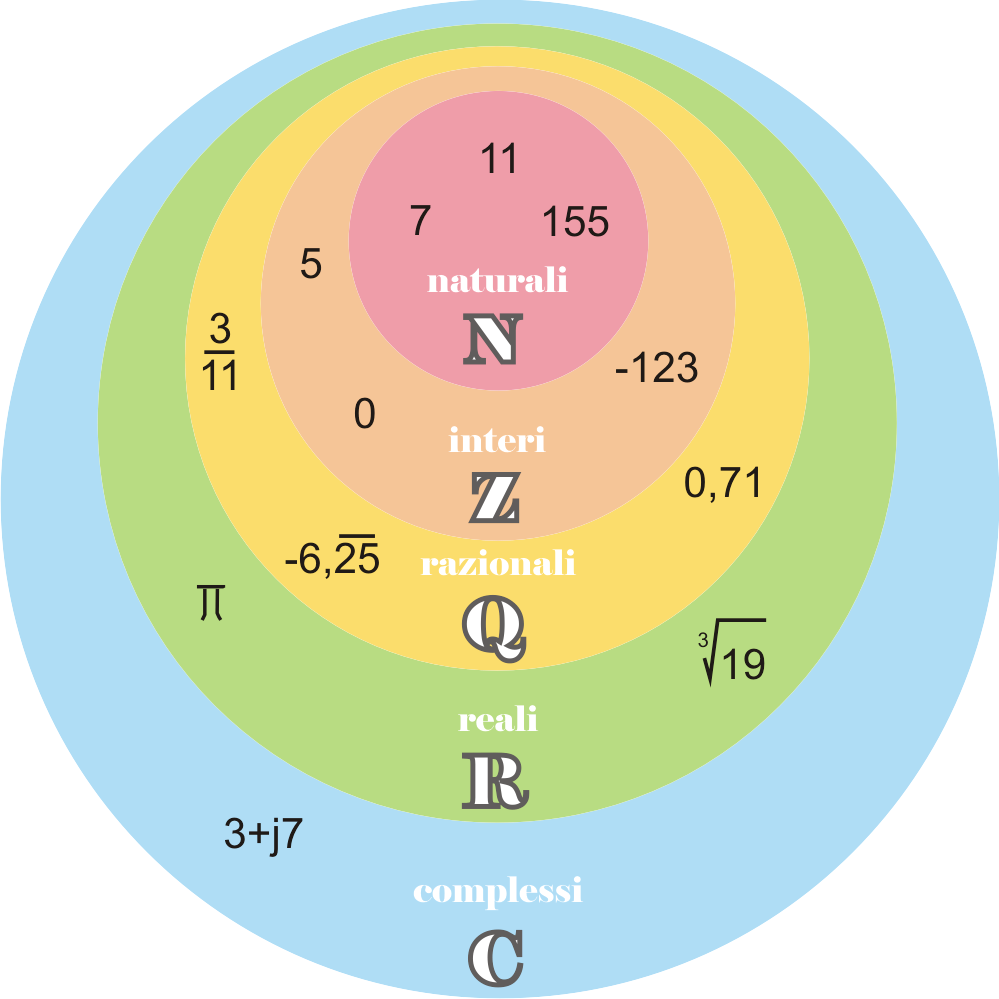
\includegraphics[width=0.5\textwidth]{insiemi_numerici.png}
        \caption{Insiemi numerici}\label{fig:insiemi_numerici}
\end{figure}


\subsection{Insiemi Indiciati}\label{sec:insiemi_indiciati}
Un \textbf{Insieme indiciato} è una famiglia di insiemi definiti da un indice $i \in I$ dove $I \in \mathbb{N}$, infatti potenzialmente $I = \{1,2,3,\ldots,n\}$. \par
Scriviamo un insieme indicato come:
\begin{equation}\label{eq:famiglia_insiemi_indiciati}
        \mathcal{F} = {\{A_i\}}_{i \in I}
\end{equation} 
Dove $\mathcal{F}$ è la famiglia, $A_i$ è l'insieme e $i$ l'indice dell'insieme. \newline
Un insieme $A_i$ ha una certa proprietà che viene ripetuta per tutti gli $A_i$ presenti nella famiglia, possiamo infatti immaginare la famiglia~\ref{eq:famiglia_insiemi_indiciati} come l'unione degli insiemi indiciati che contiene:
\begin{equation*}
        \bigcup_{i \in I}A_i = \{P(x)\}
\end{equation*}
Se avessimo $I = \{1,2,3,4,5\}$ sarebbe come scrivere:
\begin{equation*}
        A_1 \cup A_2 \cup A_3 \cup A_4 \cup A_5
\end{equation*}


\subsection{Insiemi Indiciati}
\todo{Aggiungere teoria degli insiemi indiciati}

Facciamo un esempio, prendiamo $A_i = \{x \in \mathbb{N} : x \not = 2i\}$ con $I = \{1,2,3\}$, avremo che:
\begin{itemize}
        \item $A_1 = \{\mathbb{N} \not = 2\}$
        \item $A_2 = \{\mathbb{N} \not = 4\}$
        \item $A_3 = \{\mathbb{N} \not = 6\}$
        \item $A_1 \cup A_2 \cup A_3 = \mathbb{N}$ oppure $\mathcal{F} = {\{A_i\}}_{i \in I} = \mathbb{N}$
        \item $A_1 \cap A_2 \cap A_3 = \{\mathbb{N} \not = 2, \mathbb{N} \not = 4, \mathbb{N} \not = 6\}$
\end{itemize}

Prendete con le pinze questa definizione, ma potremo immaginare gli insiemi indiciati come array di array che hanno le stesse proprietà.


\newpage
\section{Relazioni e Funzioni}
Gli elementi appartenenti a uno o più insiemi possono essere collegati attraverso diversi tipi di relazioni, per esempio i membri di una famiglia sono collegati tra loro attraverso una relazione di parentela. \par

\subsection{Relazioni}
In matematica una relazione può essere espressa attraverso $ a \to b$ oppure $ a R b $ dove $ a $ e $ b $ sono elementi di un certo insieme ed $ R $ è una relazione. \par
Questo tipo di relazione tra $ a $ e $ b $ si dice \textbf{Relazione binaria} e significa che la coppia $ (a,b) \in R $. \par

\begin{figure}[h]
        \centering
                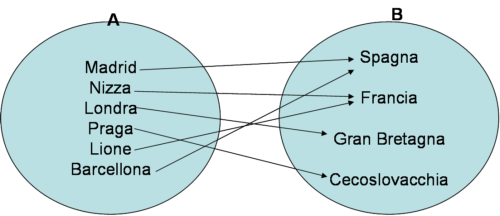
\includegraphics[width=0.75\textwidth]{relazioni.png}
        \caption{una relazione geografica}\label{fig:esempio_relazione}
\end{figure}

Altri tipi di relazioni sono:
\begin{itemize}
        \item \underline{Relazione vuota}: se $ R = \emptyset \subseteq X*Y $ 
        \item \underline{Relazione totale}: se $ R = X*Y $ 
        \item \underline{Relazione diagonale}: se $ X=Y $ in particolare viene definita con: \newline $ \Delta := \{(x,x) \in X*X\} = \{(x_1,x_2) \in X*X : x_1 = x_2\} $  
\end{itemize}
Facciamo un esempio di relazione diagonale: \newline
Prendiamo un insieme $ X = \{1,2,3\} $ avremo $ \Delta = \{(1,1), (2,2),(3,3)\} $ come relazione diagonale su $ X $.


\subsection{Funzioni}
Una funzione è anch'essa una relazione tra elementi di insiemi ma questo tipo di relazione deve rispettare questa prorpietà:
\begin{equation}\label{eq:prop_funzione}
        f \subseteq X*Y : \forall x \in X \quad \exists! y \in Y : (x,y) \in f 
\end{equation}
E si può denotare brevemente con:
\begin{equation*}
        f : X \to Y
\end{equation*}
Dove $ X $ è il detto \textbf{Dominio} e $ Y $ è detto \textbf{Codominio}. \par  
Inoltre possiamo evitarci la scrittura $ (x,y) \in f $ scrivendo semplicemente $ y = f(x) $ dicendo che $ y $ è l'immagine di $ x $ mediante $ f $. \par   

\begin{figure}[h]
        \centering
                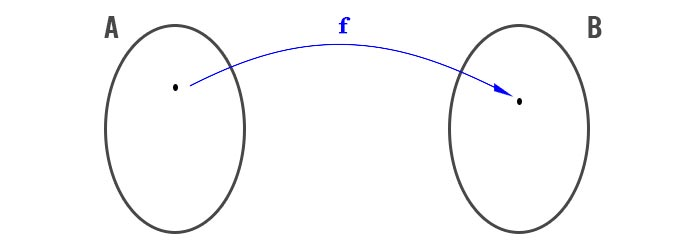
\includegraphics[width=0.75\textwidth]{esempio_funzione.jpg}
        \caption{rappresentazione di una funzione}\label{fig:esempio_funzione}
\end{figure}
Facciamo un esempio di cosa è una funzione e di cosa non lo è: \newline
Prendiamo $ X = \{1,2,3\} \quad  Y = \{a,b,c,d,e,f\} \quad $  e $\quad  \varphi, \rho \subseteq X*Y$, ipotiziamo che:
\begin{itemize}
        \item $ \varphi = \{(1,a), (1,d), (2,e), (3,a)\} $ 
        \item $ \rho = \{(1,c), (2,c), (3,a)\} $ 
\end{itemize}

Da questo possiamo di con certezza che:
\begin{itemize}
        \item $ \varphi$ non è una funzione in quanto non rispetta~\ref{eq:prop_funzione} infatti troviamo che per $ x = 1 $ esistono due $ y $ differenti. 
        \item $ \rho $ è una funzione in quanto rispetta~\ref{eq:prop_funzione}, infatti ogni $ x $ ha un solo corrispettivo $ y $.     
\end{itemize}

Aggiungo che la funzione $ \rho $ ha una $ y $ a cui corrispondono due $ x \quad $ ($ (1,c), (2,c) $) questo però non viola~\ref{eq:prop_funzione} in quanto è $ x $ che deve rispettare quella proprietà non $ y $.  


\subsection{Immagine e controimmagine}
Definiamo ora cosa sono l'immagine e la controimmagine di una funzione

\subsubsection{Immagine}
L'immagine della funzione è semplicemente la funzione stessa $ y = f(x) $ scritto anche:
\begin{equation*}
        f(A) := \{y \in Y, \exists x \in A : y = f(x) \}
\end{equation*}
Dove $ A \subseteq X $ ovvero $ A $ sottoinsieme del dominio. \newline  
\todo{Aggiungere definizione di Immagine}

\subsubsection{Controimmagine}
La controimmagine sono invece gli elementi del \textbf{codominio} $ Y $ che vengono mandati nel \textbf{dominio} $ X $. \par 
Scritto in \textit{matematichese}:
\begin{equation*}
        {f}^{-1}(B) = \{ x \in X : f(x) \in B  \}
\end{equation*}
 
Prendiamo come esempio un insieme $ X = \{1,2,3\}$ e un insieme $ Y = \{a,b,c,d,e,f\} $  e una funzione che dice:
\begin{align*}
        \varphi : X \to Y \\
        \quad 1 \mapsto c \\
        \quad 2 \mapsto c \\
        \quad 3 \mapsto a \\
\end{align*}

E prendiamo tre insiemi che sono \textit{singoletti}~\ref{def_singoletto}, $ B = \{a\} \quad E = \{c\} \quad F = \{d\}$, avremo che:
\begin{itemize}
        \item $ B = \{a\} \Rightarrow {f}^{-1}(B) = {3} $ in quanto $ a \in Y $. 
        \item $ E = \{c\} \Rightarrow {f}^{-1}(E) = {1,2}$ in quanto $ c \in Y $.  
        \item $ F = \{d\} \Rightarrow {f}^{-1}(F) = {\emptyset} $ in quanto $ d \not \in Y $.
\end{itemize}


\subsection{Iniettività, Surgettività e Bigettività}
Una funzione può essere \textbf{iniettiva, surriettiva e bigettiva}, ora spieghiamo cosa significa:
\begin{itemize}
        \item \underline{Iniettiva}: quando $ \forall x_1,x_2 \in X \quad \mbox{per cui} \quad f(x_1)=f(x_2) \Rightarrow x_1=x_2  $.   
        \item \underline{Surriettiva}: quando $ \forall y \in Y  \exists x \in X : f(x) = y $.   
        \item \underline{Bigettiva}: quando la funzione è sia iniettiva che surriettiva.  
\end{itemize}


\subsection{Il grafico della funzione}


\subsubsection{Funzione Identità}
La funzione \textbf{Identità (o funzione identica)}, è una funzione che associa ad ogni valore di $ x $ se stessa \par
Per esempio $ y=x $ o $ y = x + 0 $ sono funzioni identità. \newline
Noi scriviamo la funzione identità come:
\begin{align*}
        Id_x : X \to X \\
        \quad x \mapsto x
\end{align*}

Facciamo un esempio di funzione identità, prendiamo:
\begin{align*}
        Id_{\mathbb{N}} : \mathbb{N} \to \mathbb{N} \\
        \quad n \mapsto n
\end{align*}

Se prendiamo per esempio $ 1 \in \mathbb{N} $ avremo $ Id(1) = 1 $ \par
La funzione identità è \textbf{sempre bigettiva}.
\begin{figure}[h]
        \centering
                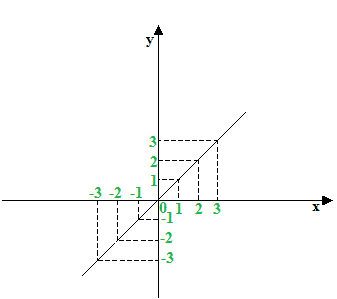
\includegraphics[width=0.75\textwidth]{es_funz_identita.png}
        \caption{La bisettrice del 1 e 3 quadrante è una funzione identità}\label{fig:esempio_funzione_identità}
\end{figure}


\subsubsection{Funzione Parte Intera}
La \textbf{funzione parte intera (o funzione floor)} è una funzione che si indica con $ \lfloor x \rfloor $ che associa ad ogni numero $ \mathbb{Z} $  il numero stesso e ad un numero decimale, l'intero precedente. \par
In matematichese questo si definisce come:
\begin{equation*}
        \forall x \in \mathbb{R} \forall n \in \mathbb{Z} \quad n \le n \Rightarrow n \le P(x)
\end{equation*}
Dove $ P(x) $ è il più grande intero $ \le  x$. \par
Facciamo qualche esempio: 
\begin{itemize}
        \item $ P(\frac{3}{2}) = 1$ perchè $ \frac{3}{2} = 1,5 $ dove $ 1 $ è la parte intera.   
        \item $ P( - \frac{1}{2}) = -1$ perchè $ - \frac{1}{2} = -0,5 $ dove in questo caso è $ -1 $ l'intero più vicino. 
\end{itemize} 


\begin{figure}[h]
        \centering
                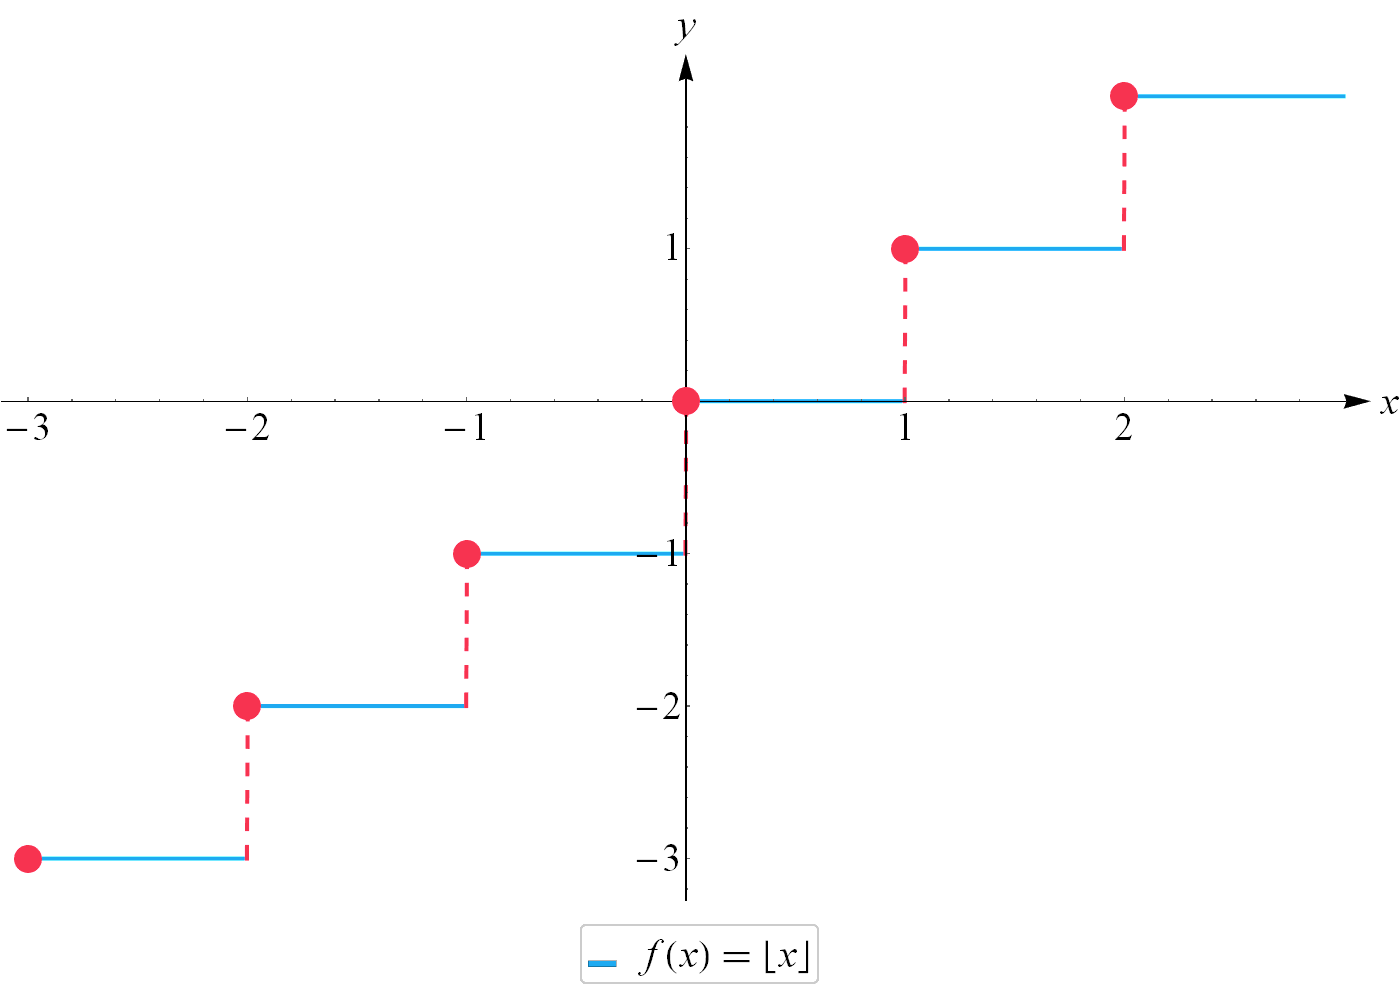
\includegraphics[width=0.75\textwidth]{esempio_funzione_parte_intera.png}
        \caption{Esempio di funzione parte intera}\label{fig:esempio_funzione_parte_intera}
\end{figure}


\subsubsection{Funzione Parte Frazionaria}




\subsubsection{Funzione Composta}
\subsection{Invertibilità}

\newpage
\section{Assioma della scelta}



\newpage
\section{Principio di Induzione}
Il \underline{Principio di induzione} detto anche procedimento induttivo è un procedimento matematico per dimostrare la validità di una tesi attraverso la verifica della veridicità di due condizioni:
\begin{itemize}
        \item \underline{passo zero}: $(n_0)$
        \item \underline{passo induttivo}: $(n)$
\end{itemize}
Se lo scriviamo in matematichese diciamo che se abbiamo una proposizione $P$ e:
\begin{align*}
        P(n_0) \quad \mbox{vera} \\
        P(n) \quad \mbox{vera}
\end{align*}
Allora $P(n)$ è vera. \par
Ne consegue quindi che anche $P(n+1)$ è vera, potremo dire semplicemente che se:
\begin{equation*}
        P(n) \quad \mbox{vera} \quad \Rightarrow \quad P(n+1) \quad \mbox{vera}
\end{equation*}

Utiliziamo un esempio, dimostramo che $\forall n \ge 0$ la somma che denotiamo con $S(n)$ dei primi numeri naturali:
\begin{equation*}
        S(n) = 0 + 1 + 2 + 3 + 4 + 5 + \cdots + n
\end{equation*}
è data da:
\begin{equation*}
        S(n) = \frac{n(n+1)}{2} \quad \forall n \ge 1
\end{equation*}

La nostra proposizione sarà quindi:
\begin{equation*}
        P(n) : S(n) = \frac{n(n+1)}{2}
\end{equation*}

Il nostro compito sarà quindi quello di dimostrare che $P(n_0)$ e $P(n)$ è vero $\forall n \ge 1$. \par
Quindi dimostriamo $S(n)$ con $n = 1$:

\begin{equation}\label{eq:esempio_induzione_1}
        S(1) = \frac{0*(0+1)}{2} = 0
\end{equation}

A questo punto secondo la proprietà dell'induzione anche $P(n+1)$ sarà vera ovvero $S(1)$:
\begin{equation}\label{eq:esempio_induzione_2}
        S(1) = \frac{1*(1+1)}{2} = 1
\end{equation}

Esistono tre tipi di induzione che spiegheremo di seguito.


\subsection{Prima forma}
Il \underline{Principio di induzione prima forma} dice che con $P$ proposizione sui numeri naturali:
\begin{enumerate}
        \item $P(0)$ è vera. 
        \item $P(n)$ è vera $\Rightarrow P(n)$ vera allora $P(n)$ vera $\forall n \in \mathbb{N}$. 
\end{enumerate}
Un esempio di ciò è~\ref{eq:esempio_induzione_1} e~\ref{eq:esempio_induzione_2}.


\subsection{Seconda forma}
Il \underline{Principio di induzione seconda forma} dice che con $P$ proposizione sui numeri naturali e $n_0 \in \mathbb{N}$ dove $n_0$ è il \textbf{passo zero}, se vale:
\begin{enumerate}
        \item $P(n_0)$ vera.
        \item $P(n)$ vera $\Rightarrow P(n+1)$ vera.
\end{enumerate}
Allora $P(n)$ è vera $\forall n \ge n_0$.

\subsection{Terza forma}
Il \underline{Principio di induzione terza forma} dice che con $P$ proposizione su $\mathbb{Z}$ e $n_0 \in \mathbb{Z}$ dove $n_0$ è il \textbf{passo zero}, se vale:
\begin{enumerate}
        \item $P(n_0)$ vera. 
        \item $P(n)$ vera $\forall m \in \mathbb{Z} \quad n_0 \le m < n \Rightarrow P(n)$ vera. 
\end{enumerate}
Allora diciamo che $P(n)$ vera $\forall n \ge n_0$.




\newpage
\section{Esempio}
Se considero la funzione:
\begin{align}
        f :  \mathbb{Z}^{2} \rightarrow \mathbb{Z} \\
        (x,y) \rightarrow 21x - 15y
\end{align}
Dobbiamo dimostrare che la funzione è \textbf{iniettiva} o \textbf{surriettiva}.
Prendiamo quindi $f(1,1) = 21 - 15 = 6$ possiamo dire che \newline
$f \textrm{surriettiva} \Leftrightarrow f(\mathbb{Z}^{2}) = 2$
e che quindi:
$f(\mathbb{Z}^{2}) = {n \in \mathbb{Z} : \exists(x,y) \in \mathbb{Z}^{2} n=f(x,y)=21x - 15y} $

Quella che abbiamo appena scritto è una funzione \textbf{Diofantea} ovvero $MCD(21,15) : n \Leftrightarrow f(\mathbb{Z}^{2})={3k : k \in \mathbb{Z}}$. \par

E quindi possiamo dire con certezza che la funzione non è né surriettiva e né iniettiva perchè:
\begin{align*}
        1 \notin f(\mathbb{Z}^{2}) \\
        \textrm{Perchè fissato } & n \in 3Z
\end{align*}







\newpage
\section{Numeri Primi}
\textit{I numeri primi sono quei \textbf{numeri interi maggiori di 1 che sono divisibili solo per 1 e se stessi}, se questa proprietà non viene rispettata allora il numero è invece \textbf{composto}} che scritto in matematichese:
\begin{align}
       a \in \mathbb{Z}, a>1
\end{align}

Dimostramo ora un \textbf{Lemma} dei numeri primi:

\begin{align}
        a,b \in Z, p \in Z \quad \textrm{Primo} \\
        p | a \quad \textrm{o} p | a*b
\end{align}
Quindi supponiamo di avere $p T a$, dimostriamo che $p|b$
$p | a*b \Rightarrow \exists k \in Z$ tale che $a*b = k*p$

Possiamo dimostrarlo utilizzando anche \textbf{Bezout} (DA FARE A CASA).


\subsection{Teoria fondamentale dell'aritmetica}
Ok prepariamoci a scrivere un pò di formule. \newline
si dice che: $a \in Z, a \not = 0,1,-1$ allora $a$ si scrive in un modo unico come prodotto di primi:
\begin{equation}
a =
\end{equation}


\subsection{Teorema di euclide}
Esistono infiniti numeri primi e lo possiamo dimostrare attraverso una dimostrazione per assurdo.
Supponiamo infatti per assurdo che esistano soltato $p_1,\ldots,p_n$ numeri primi. \par
Perfetto ora consideriamo un numero $N = p_1* \ldots * p_n$.
La divisione euclidea di $N$ per $p_1$ da resto 1.
Analogamente $N$ diviso per $N = p_1* \ldots * p_n$ da resto $1$ \par

$p_1 \dag N$ \ldots  $p_n \dag N$ contraddice il teorema precedente e perciò abbiamo dimostrato che ci sono infiniti numeri primi, ok può non essere chiarissimo quindi vado ad utilizzare i numeri per fare un esempio:
\begin{align*}
        N = 2 * 7 + 1 = 14 + 1 = 15 \quad \textrm{Non è primo} \\
        3 | 15, 5 | 15
\end{align*}
Abbiamo infatti trovato due nuovi numeri primi 3 e 5 quindi ci sono infiniti numeri primi.




\newpage
\section{Numeri complessi}\label{sec:numeri_complessi}
Noi definiamo numeri complessi quei numeri che


$C = R x R$ denotiamo che $(x,y) \in R^2$ come $x + iy$ e consideriamo $i$ come unità immaginaria, definiamo due operazioni su C
\begin{itemize}
        \item \textbf{Somma} $(x + iy) + (u + iv) := (x+u) + i(y+v)$ con $x,y,u,v \in R$
        \item \textbf{Prodotto} $(x + iy) * (u + iv) := (xu - yv) + i(xv+yu)$ con $x,y,u,v \in R$
\end{itemize}

Utiiziamo un esempio numerico:
\begin{align}
        \textrm{Somma: } \quad (2 + 3i) + (4 + 5i) = (2 + 4) + i(3 + 5) = 6 + 8i \\
        \textrm{Prodotto: } \quad (2 + 3i) + (4 + 5i) = (2 * 4) + i(2*5 + 3*4) = (8-15 + i(10+12)) = 7 + 22i
\end{align}

Anche se i calcoli possono sembrare complssi possiamo semplificare il tutto con questo ragionamento:
\begin{equation}
        i + i = (0*0 - 1*1) + i(0+1 + 0+1) = -1+ i0 = -1
\end{equation}

L'inverso di $x + iy$ rispetto al punto si denota con ${(x + iy)}^{-1}$ oppure $\frac{1}{x + iy}$


\subsection{Piano di Gauss}
Con $\mathbb{C} = \mathbb{R}^2$ consideriamo un piano cartesiano possiamo rappresentare tutti i numeri complessi utilizzando però delle coordinate dette \textbf{Polari}.
Da un punto $x$ e un punto $y$ troviamo un punto $z$ possiamo infatti dire che $z = x+iy$ dove il $|z|$  rappresenta la distanza del punto $z$ dall'origine (l'intersezione dell'asse x e y) e lo si può calcolare attraverso \textbf{Pitagora} con $|z| := \sqrt{x^2+y^2}$. \par
E quindi se $z \in \mathbb{R}$ allora $|z| = \sqrt{x^2}$

\subsection{Proprietà dei numeri complessi}

\begin{itemize}
        \item $\overline{zw} = z * \overline{w}$ \\
        \item $\overline{z} = z$ \\
        \item $\overline{z+w} = \overline{z} + \overline{w}$ \\
        \item $z+\overline{z}=2Re(z)$ \\
        \item $z - \overline{z}=2Im(z)$ \\
\end{itemize}
Cercare le dimostrazioni su internet perchè oggi il prof ha deciso di fare il cosplay di Flash.

Altre proprietà però con il modulo:
\begin{itemize}
        \item $z * \overline{z} =   |z|^{2}$ \\
        \item $|zw| = |z| |w|$ \\
        \item $|z+w| \le |z| + |w|$ \\
        \item $z \not = 0 \quad z^{-1} = \frac{\overline{z}}{|z|^{2}} $ \\
\end{itemize}

\textbf{CERCARE SU INTERNET DISUGUAGLIANZA TRIANGOLARE E GRAFICO CON IL MODULO} \newline

$\theta = \arg(z)$
argomento di z angolo formato da z e l'asse $Re$ $\theta$ è definito a meno di $Re$ multipli di $2\pi$

\textbf{CERCARE SU INTERNET FORMA TRIGONOMETRICA Z} \newline

Ok facciamo un esempio, prendiamo $z = 2$, avremo quindi $|z| = \sqrt{2^2 = 2}$ e $\arg{z} = 0$.\par
A questo punto possiamo dire che $z = 2(\cos(0) + i\sin(0))$ \newline

\textbf{RICORDARSI CHE Re STA PER PARTE REALE (GRAZIE GABRIEL DEL PASSATO)} \newline


\subsection{Forma esponenziale}
Avendo $z \in \mathbb{C}, z \not = 0$ \newline
$\theta = \arg z$ e  $z = | z | e^i*\arg(z)$ \newline
$w \in \mathbb{C}, w \not = 0 := |z| (\cos(\theta) + i\sin(\theta))$ \newline

\textbf{CERCARE FORMULA DI DE MOUIURE}


\subsection{Equazioni di secondo grado complesse}
Una radice semplice si calcola quando si hanno equazioni di grado inferiore al terzo, nello specifico ogni equazione di secondo grado $ax^2+bx+c = 0$ con $a,b,c \in \mathbb{C}$ ha due soluzioni in $\mathbb{C}$. \par
Si trovano così  $\Delta := b^2 - 4ac$ dove:
\begin{itemize}
        \item $\Delta = 0 \quad \mbox{prendo} \quad \delta_1 = \delta_2 = 0$	
        \item $\Delta \not = 0 \quad \mbox{per il teorema} \quad \exists \delta_1,\delta_2 \in \mathbb{C} \quad \mbox{distinti, tali che} \quad \delta_1^2 = \delta_2^2 = \Delta$	
\end{itemize}

Le soluzioni dell'equazione di secondo grado si trovano facendo:
\begin{align}
        z_1 = \frac{-b + \delta_1}{2a} \\
        z_1 = \frac{-b + \delta_2}{2a} 
\end{align}

Mentre:
\begin{align}
        \mbox{Se} \quad \Delta = 0, \delta_1=\delta_2 \quad \mbox{quindi} \quad z_1=z_2 \\
        \mbox{Se} \quad \Delta < 0, \delta_1 \not = \delta_2 \quad \mbox{quindi} \quad z_1 \not = z_2 
\end{align}


\subsection{Radici complesse}
le $Zk$ sono chiamate radici complesse che se le andassimo a disegnare sul piano di Gauss formerebbero i su \newline

Facciamo un esempio, le radici cubiche $(n=3)$ di $z = -8 +i*0$ del modulo di $z, \quad|z| = \sqrt{Re(z^2)+In(z^2)} = \sqrt{-8^2 + 0^2} = \sqrt{(-8^2)} = 8$.


\subsection{Teorema fondametale dell'Algebra}
Il teorema fondamentale dell'algebra dice che ogni polinomio in $\mathbb{R}$ o $\mathbb{C}$ di grado $\geq 1$ ha soluzioni nei $\mathbb{C}$ \newline 
Ovvero sia $p(x) = a_n X^n + a_{n-1} X^{n-1} + \cdots + a_1 X + a_0$ un polinomio, $p(x) = a_n  + a_{n-1} + \cdots + a_1 + a_0 \in \mathbb{C} a_n \not = 0$ di grado $n$ \par
Allora $p(x)$ ha $n$ soluzioni in $\mathbb{C}$ contate con la loro molteciplità.\par
Cioè $p(x)$ si può decomporre come $p(x) = {a_(x-w_1)}^{m_1} \cdots {(x-w_r)}^{m_r}$ \newline

(a detta del prof è troppo complesso dimostrarlo e se lo dice lui io mi fido)





\newpage
\section{Relazioni di Equivalenza}
Prima di tutto definiamo un insieme $A$, una relazione $R \subseteq AxA$ si dice di equivalenza se soddisfa:

\begin{enumerate}
        \item \underline{Riflessiva} ($\forall a \in A (a,a) \in \mathbb{R})$
        \item \underline{Simmetrica} ($(a,b) \in \mathbb{R} \Rightarrow (b,a) \in \mathbb{R}$)
        \item \underline{Transitiva} ($(a,b) \in \mathbb{R},(b,c) \in \mathbb{R} \Rightarrow (a,c) \in \mathbb{R}$)
\end{enumerate}


Generalmente indichiamo una relazione d'equivalenza con un simbolo  $\backsim$ oppure $\equiv$ e scriviamo $a \backsim b$ oppure $a \equiv b$ oppure $aRb$ per indicare $(a,b) \in \mathbb{R}$


\subsection{Equivalenza modulare}
$A = \mathbb{Z}$ fissiamo $n \in \mathbb{Z}, n \geq 1$ definiamo $\backsim_n$ \par
$x \backsim_n y \Leftrightarrow \exists k \in \mathbb{Z}$ tale che $x-y = Kn$ si diche che $x$ è congruo a $y$ mmodulo $n$ e si scrive $x \equiv y MOD n$.


$\forall x \in \mathbb{Z} \mbox{vale} \quad x \equiv x \mod n$ perchè $\exists K \in \mathbb{Z}$ tale che $x-x = K*n$ 


\subsection{Classe di equivalenza}
Sia $A$ un insieme e sia $\backsim$ una relazione di equivalenza su $A$. La \underline{classe di equivalenza} di un elemento $a \in A$ con $\overline{a} = [a] := \{b\in A : b \backsim a\}$ è un insieme. \par
$a$ si chiama rappresentante della classe $[a]$ e notare bene che $a \in [a]$ perchè $a \backsim a$.




\newpage
\section{Cardinalità}
Con \textbf{cardinalità} noi intendiamo definire quali e quanti elementi fanno parte di un certo insieme utilizzando il linguaggio matematico. \par

Supponiamo per esempio che $A,B$ sono insiemi, possiamo dire che $A,B$ sono \textbf{equipotenti} se $\exists f:A \rightarrow B$ bigettiva, in tal caso scriviamo $|A| = |B|$. \par

Ok detto questo mostriamo alcune proprietà:
\begin{enumerate}
        \item \textbf{Riflessiva} A è equipotente con $A$ tramite $id_A A \rightarrow A$ bigettiva.
        \item \textbf{Simmetrica} $A$ è equipotente a $B$ $\Rightarrow \exists f:A \rightarrow B$ bigettiva. 
        \item \textbf{Transitiva} $A$ equipotente a $B$, $B$ equipotente a $C$.	
\end{enumerate}

Con X insieme diciamo che:
\begin{itemize}
        \item $X$ è finito se $X = \not 0$ oppure $\exists n \in \mathbb{N}$ tale che $X$ è equivalente a $\{1,2,3,4,n\}$ e in tal caso diciamo che $X$ ha cardinalità $n$ scrivendo $|X| = n$.
        \item X è \textbf{infinito} se X non è finito (ovviamente), si dice che X insieme è $= \not 0$ allora sono equivalenti e si dice anche che:
        \begin{enumerate}
                \item$X$ è infinito
                \item $\exists Y \subsetneq X$ tale che $|Y|=|X|$.
                \item $\exists f:X \to X$ iniettiva, ma non suriettiva.
        \end{enumerate}
\end{itemize}

$X$ si dice \textbf{numerabile} (o di cardinalità numerabile) se $|X| = |\mathbb{N}|$ e scriviamo $|X| = X_0$ e lo si chiama \textbf{Aleph Zero}. \par
Se $X$ è numerabile $\Rightarrow X$ infinito. \newline
$f \circ s \circ f^{-1} X \rightarrow X$ iniettiva, ma non surriettiva.

Esempio proviamo a vedere se $\mathbb{Z}$ che contiene $\mathbb{N}$. \par
\begin{equation}
        f : \mathbb{N} \rightarrow \mathbb{Z}
\end{equation}
ok ora vediamo che: \newline

\[
f(n) =
\begin{cases}
        \frac{n}{2} \quad \mbox{se $n$ è pari} \\
        \frac{n + 1}{2} \quad \mbox{se $n$ è dispari}
\end{cases}
\]

se invece $f$ è bigettiva, l'inversa è $f^{-1}: \mathbb{Z} \to \mathbb{N}$


$\mathbb{N} x \mathbb{N}$ è numerabile dimostriamo che $f: \mathbb{N} x \mathbb{N} \to \mathbb{N}$.

\textbf{AGGIUNGERE ESEMPI}.

Definiamo $A,B$ insiemi e scriviamo: 
%\begin{itemize}
%        \item $|A| \le |B|$ se $\exists f:A \to B$ iniettiva.
%        \item $|A| < |B|$ se: $|A| \le |B|$ ($\exists f:A \to B)$ iniettiva. $|A| \not = |B|$ ($\not \exists f:A \to B)$ iniettiva$
%\end{itemize}

\textbf{Altra parte di lezione mancante}

\subsection{Teorema di Cantor-Bernstein}
$A,B$ insiemi, $\exists f : A \to B$ iniettiva, $g: B \to A$ iniettiva, allora esiste una funzione $\exists h: A \to B$ bigettiva. \par
In formule questo ci dice che se:
\begin{equation}
        |A| \le |B| \quad |B| \le |A| \Rightarrow |A| = |B|
\end{equation} \newline

Se $A,B$ finiti, $|A| = n, \quad |B|= m \quad n,m \in \mathbb{N}$ allora: 

\[n=m :
\begin{cases}
        |A| \le |B| \Rightarrow n \le m \\
        |B| \le |A| \Rightarrow m \le n
\end{cases}
\]


Definiamo $X$ insieme, diciamo che:
\begin{itemize}
        \item X è \underline{al più numerabile} se $|X| \le |\mathbb{N}|$	
        \item X è \underline{più che numerabile} se $|X| > |\mathbb{N}|$
\end{itemize}

\textbf{PROBABILMENTE C'È TROPPA ROBA CHE NON HO SCRITTO} \newline


\subsection{Impossibilità della surriettività dei numerabili}
Prendiamo la proposizione che prende $X$ insieme con $X \not =  \not 0$ allora non esite alcuna mappa surriettiva $X \to P(x)$ \par
In particolare questo ci dice che $|X| \not = |P(x)|$ e quindi $X$ e $P(x)$ non sono equipotenti.

Bene proviamo a dimostrare quello che abbiamo appena detto per assurdo, supponiamo infatti per assurdo che $\exists f : X \to P(x)$ surriettiva e prendiamo un insieme $S = {x \in X : x \not \in f(x)}$. \par 
Abbiamo che:
\begin{itemize}
        \item $S \subseteq X$, Eventualmente $S$ può essere $\emptyset$.
        \item $S \in P(x)$ ed essendo $f$ surgettiva $\exists s \in X$ tale che $f(s) = S$ 
\end{itemize}
Quindi la domanda è $s \in S$ o $s \not \in S$, andiamo a trovare la contraddizione:
\begin{enumerate}
        \item Se $s \in S$ allora $s \not \in f(s) = S$ che è una \textbf{CONTRADDIZIONE}.
        \item Se $s \not \in S$ allora $s \in f(s) = S$ che è anch'essa una \textbf{CONTRADDIZIONE}.
\end{enumerate}

Da tutto questo osserviamo che $X \not = \emptyset \exists f : X \to P(x)$ iniettiva e cioè $f(x) = {x}$ (il singoletto composto da x) e ciò implica che $\Rightarrow |X| \le |P(x)|$. 

La proposione precedente ci dice che $|X| < |P(x)|$ ad esempio per $X = \mathbb{N}$ si ha: \newline
$|P(\mathbb{N})| > |\mathbb{N}| = \aleph_0 $ dove $P(\mathbb{N})$ è più che numerabile.

\subsection{Argomento che il prof si tiene segreto}
Definiamo $A,B$ insiemi.
\begin{equation}
        B^A := {f:A \to B \quad \mbox{funzione}}
\end{equation}
E nel caso in cui $B = {0,1}$ si usa indicare ${0,1}^A$ con $2^A$.


Vogliamo $X$ insieme dove $X \not = \emptyset$ allora $P(x)$ è equipotente a ${0,1}^x$. \newline
$|P(x)| = |{0,1}^x|$.

Dimostriamo (quello che ho scritto senza sapere cosa stavo scrivendo) con:
\begin{align*}
        \phi : {0,1}^x \to P(x) \\
        f \mapsto {f(1)}^{-1} = \{x \in X : f(x) = 1\} \subseteq X
\end{align*}

Iniziamo con le dimostrazioni:
\underline{$\phi$ surriettiva} sia $A \in P(x), A \subseteq X$ sottoinsieme e considero $X_A : X \to {0,1}$.



\[x \mapsto  
\begin{cases}
        1 \quad \mbox{se} \quad x \in A \\
        0 \quad \mbox{se} \quad x \not \in A \\
\end{cases}
\]

\begin{align*}
X_A \in {0,1}^X \\
\varphi(X_A) = {X_A}{-1}(1) = \{x \in X : X_A(x) = 1\} = \{x \in X : x \in A\} = A.
\end{align*}

Ora che non so che cazzo ho scritto prendiamo $\phi$ iniettiva e $f,g \in {0,1}^x, f \not = g$ tesi $\phi(f) \not = \phi(g)$.
$f,g : X \to {0,1}$ \newline
$f \not = g \Rightarrow \exists x \in X$ tale che $f(x) \not = g(x)$.
Supponiamo che $f(x) = 1 \Rightarrow g(x) = 0$ \newline
$\Rightarrow x \in {f}{-1} = \varphi(f) x \not \in {g}{-1}(1) = \varphi(g) \Rightarrow \varphi(f) \not = \varphi(g)$

\textbf{MA CHE CAZZO HO APPENA SCRITTO} \newline


Prendiamo il lemma $A = {a_1,\ldots,a_n}$ insieme finito, $B$ insieme finito, $|B^A| = |B^n|$ che (a quanto dice il prof) è facilmente dimostrabile:
\begin{align*}
         \varphi : B^A \to B^n = Bx,\ldots,xB \\
                   f \mapsto (f(a_1),\ldots,f(a_n))
\end{align*}

Corollario $A,B$ insiemi finiti, allora $AxB, B^A, P(A)$ sono insiemi finiti di cardinalità:
\begin{itemize}
        \item $|A*B| = |A|*|B|$	
        \item $|B^A| = |B|^{|A|}$
        \item $P(A) = |{0,1}^A| = |\{0,1\}|^{|A|} = 2^{|A|}$	
\end{itemize}


\subsection{Cardinalità dei $\mathbb{Q}$}

Prima di tutto diciamo che $\mathbb{Q}$ è numerabile, e lo possiamo dimostrare con:
\begin{align*}
        \varphi : \mathbb{Q}\{0\} \to \mathbb{N}* \\
        \frac{p}{q} \mapsto |p| + |q|
\end{align*}

Avendo $p,q \in \mathbb{Z}, p,q \not = 0, MCD(p,q)=1$ e quindi, $Q = {0} \cup \bigcup_{n \in \mathbb{N}}{\varphi^{-1}(n)}$.

Si dice quindi che \underline{unione numerabile} di insiemi finiti $\not = 0$ e disgiunti $\Rightarrow Q $ numerabile. \newline

\textbf{Cercare la diagonale di Cantor}

\underline{Lemma} prendiamo $\{X_m : m \in \mathbb{N}\}, |X_n| \le \aleph_0, X_m \not = \emptyset \forall n \in \mathbb{N}$ se $|Xm| < \aleph_0 \forall n \in \mathbb{N}$ allora $X_n \cap X_m = \emptyset$ se $n \not = m$ allora $|\bigcup_{n \in \mathbb{N}}^{1}X_n| = \aleph_0$ \newline


\subsection{Cardinalità di $\mathbb{R}$}
$ \mathbb{R}$ è equipotente a $P(\mathbb{N})$, in particolare è più che numerabile. \par

\begin{align*}
        \mbox{Cardinalità} \quad 0,1,2,\ldots n\ldots,\aleph_0 \\
        \mbox{Insiemi} \quad \emptyset, {*}, {1,2}, \ldots, {1,\ldots,n},\ldots,\mathbb{N},\mathbb{Z},\mathbb{Q},\ldots        
\end{align*}


\subsection{Ipotesi del continuo}
Questa ipotesi, formulata da \underline{Cantor} chiede se $ \exists A$ insieme tale che $\aleph_0 < |A| < 2^{\aleph_0}$?? 

\textit{BTW questi problemi non verrano trattati nel corso ma sono good to know}.




\newpage
\section{Calcolo Combinatorico}

Iniziamo con una definizione, se abbiamo $X$ insieme infinito, \par ovvero: $\{X \to X \quad \mbox{Bigettiva}\}$ è l'insieme delle \underline{permutazioni di $X$}, nel caso in cui $X = \{1,\ldots, n\}$, l'insieme è detto \textbf{Insieme delle permutazioni} si denota con:
\begin{equation*}
        S_n = \{\{1,\ldots, n\} \to \{ 1,\ldots,n\} \quad \mbox{Bigettiva}\}.
\end{equation*}

E con il \textit{lemma} $X,Y$ insiemi finiti, $|X| = n \le m = |Y|$ Il numero delle applicazioni iniettive $X \to Y$ è uguale:
\begin{equation*}
        m * (m-1)*\ldots*(m-n+1)
\end{equation*}

Osserviamo che se $n > m, \not \exists X \to Y$ iniettiva, facilmente dimostrabile con $|X| = n \Rightarrow X = \{x_1,x_2,\ldots,x_n\}$. \par
Possiamo vedere in quanti modi possiamo definire $f:X \to Y$ iniettiva. 
Prendimo $X = \{x_1,\ldots,x_n\} \to Y = \{y_1,\ldots,y_n\}$:
\begin{itemize}
        \item $x_1 \mapsto \mbox{?}$ ho $m$ possibili scelte.
        \item $x_2 \mapsto \mbox{?}$ ho $m-1$ possibili scelte.
        \item $x_3 \mapsto \mbox{?}$ ho $m-2$ possibili scelte.
        \item $x_n \mapsto \mbox{?}$ ho $m-(n-1)$ possibili scelte.
\end{itemize}

In tutto quindi avremo $m(m-1),\ldots,(m-n+1)$ possibili funzioni $X \to Y$ iniettive $\square$. \par

Corollario $|X| = |Y| = n$ ci sono $n(n-1),\ldots,(n-n+1) = n(n-1),\ldots,(2)$ funzioni bigettive da $X$ a $Y$. \par
Definiamo $n \in \mathbb{N}$, il \underline{fattoriale} di $n$:
\[ n! = 
\begin{cases}
        n * (n-1) * \ldots * 2 * 1 \quad \mbox{se} \quad n>0\\
        1 \quad \quad \mbox{se} \quad n = 0
\end{cases}
\]

Un altro corollario, $|S_n| = n$! che definiamo con:
\begin{align*}
        n,k \in \mathbb{N}, n \ge 1, 0 \le k \le n, \quad \mbox{\underline{il coefficiente binomiale}} \\
        (n k) := \frac{n!}{k!(n-k)!}
\end{align*}



\subsection{Mi inventerò un titolo}
X insieme finito, $|X| = n$ per ogni intero $0 \le k \le n$ il numero di sottoinsiemi di $X$ con $k$ elementi è $(n su k)$.

Dimostrimolo:
\begin{itemize}
        \item $k=0$, c'è solo un insieme con 0 elementi: $\emptyset$
        \item $k=n$, c'è solo un insieme con n elementi: $(n su n) = (n su 0) = 1$
\end{itemize}


Ora proviamo a cotruire un $Y \subseteq X$ con $\#Y = k$ e $0 < k < n$ \par
\begin{itemize}
        \item Scegliamo il 1° elemento di $y$:$n$ possibilità
        \item Scegliamo il 2° elemento di $y$:$n-(k-1)$ possibilità
\end{itemize}

Devo dividere per il numero di permutazioni di una stringa con $k$ elementi:
\begin{equation*}
        \frac{n(n-1)\ldots(n-k+1)}{k!} = (n su k) \square
\end{equation*}


\underline{Lemma} $(n su k) = (n-1 su k) + (m-1 k-1)$ 


\subsection{Coefficiente binomiale}
Il coefficiente binoiale è $x,y \in \mathbb{C}, n \in \mathbb{N}*$ allora:
\begin{equation*}
        {(x+y)}^{n} = \sum_{k=0}^{n}(n su k)x^{n-k}y^k
\end{equation*}

Dimostriamolo attraverso l'induzione: \newline
\todo{Dimostrare il coefficiente binomiale attraverso l'induzione}


Corollario $X$ insieme finito, $|X| = n$ allora $|P(x)| = 2^n$ dimostrabile $\forall 0 \le k \le n$ il numero di sottoinsiemi di $k$ elementi di $X$ è (n su k). \par
Il numero di sottoinsiemi di $X$ è: 
\begin{equation*}
        \sum_{k=0}^{n}(n su k) = 2^n
\end{equation*}




\newpage
\section{Relazioni d'ordine}
Le relazioni d'ordine sono un tipo di relazione che hanno come modello la disuguaglianza per esempio tra insiemi di diverso tipo oppure oggetti che non necessariamente sono numeri. \par
Se vogliamo dare una definizione più precisa possiamo dire che se $ X $  insieme, $ R \subseteq X * X $ relazione $ R $ è un \underline{preordine} se:
\begin{itemize}
        \item \underline{Riflessiva}: $ \forall x \in X \quad (x,x) \in R$ 
        \item \underline{Transitiva}: $ (x,y) \in R \quad (y,z)  \in R \Rightarrow (x,z) \in R$ 
        \item \underline{Antisimmetrica}: $ ((x,y) \in R) \land ((y,x) \in R) \Rightarrow x = y $ 
\end{itemize}

si dice che $ R $ è un ordine parziale. \newline
In questo caso $ X $ si dice \underline{parzialmente ordinato} (POSET) \par
Scriviamo $ (x,y) \in R $ come $ x \triangle y $ oppure $ x \le y | (x, \triangle)$  dove $x$ è un insieme e $ \triangle $ è un \textbf{ordine parziale} su $ X $    

Definiamo meglio $ (x, \triangle) \quad  POSET \quad x,y \in X$, si dicono \underline{confrontabili} se vale $ (x \triangle y) \lor (y \triangle x) $, altrimenti si dicono non confrontabili  se tutti gli elementi di $ X $ sono confrontabili, $ \triangle $ si dice \underline{ordine totale}.  \par

\subsection{Esempi di relazioni d'ordine}
Prendiamo come adesso alcuni esempi: \newline 
$ \mathbb{R}, \le $ è totalmente ordinato ($ \le $ è un ordine totale su $ \mathbb{R} $) 1.:
\begin{itemize}
        \item $ x \le x \forall x \in \mathbb{R} $ \underline{Riflessiva}
        \item $ x \le y, y \le z \Rightarrow x \le z$ \underline{Transitiva}
        \item $ x \le y, y \le x \Rightarrow x=y  \mathbb{R} $ \underline{Antisimmetrica}
\end{itemize}
è totale perchè dati $ x $ \newline

2. $ < $ minore stretto non è un ordine parziale su $ \mathbb{R} $ non soddisfa la riflessiva \newline

3. $ \triangle = \{(x,y) \in X : x = y\}$ ordine parziale. \newline 

4. $ \mathbb{C} z \triangle w \Leftrightarrow |z| \le |w| $ dove $ z,w \in \mathbb{C} $  è un preordine ma, ma non un ordine parziale perchè:

\begin{itemize}
        \item \underline{Riflessiva} $ z \triangle z$ si perchè $ |z| \le |z| $
        \item \underline{Transitiva} $ x \triangle y, y \triangle z \Rightarrow x \triangle z$  si perchè $ |x| \le |y| $
        \item \underline{Antisimmetrico} no perchè prendiamo per esempio \newline $ x = i, |i| = 1 \le 1 = |1| \quad i \triangle 1 $ ma $ i \not = 1 $  \newline $ y = 1 \quad |1| = 1 \le 1 = |i| \quad 1 \triangle i $    
\end{itemize}

5. $ X $ insieme, $ X \not = \emptyset $, definiamo una relazione d'ordine su $ P(x)  A,B \in P(x) \quad \quad A \triangle B \Leftrightarrow A \subseteq B $ \par
In particolare $ (P(x), \subseteq )$ è un POSET:\newline
\begin{itemize}
        \item $ A \subseteq A $
        \item $ A \subseteq B, B \subseteq C \Rightarrow A \subseteq C $
        \item $ A \subseteq B, A \subseteq B \Rightarrow A = B $
\end{itemize}
$ \subseteq $ non è totale, esempio $ X = \{1,2,5\}, A = \{1,2\}, B = \{2,3\} $ e se $ X \not = \{*\} $


\subsection{Tipi di ordini}
Definiamo $(A_1, \triangle_1), \ldots, (A_n, \triangle_n) \quad POSET$ definimo ordini parziali su $A_1x, \ldots, xA_n$. \newline


\subsubsection{Ordine lessicografico (LEX)}
\underline{Ordine lessicografico (LEX)}:
\[ 
(a_1,a_2,\ldots, a_n) \triangle_{lex} (b_1,b_2,\ldots, b_n) \Leftrightarrow   
\begin{cases}
        a_1 \triangle_1 b_1 \quad \mbox{se} \quad  a_1 \not = b_1 \\
        a_{k+1} \triangle_{k+1} b_{k+1} \quad \mbox{se} \quad  a_j = b_j \forall j = 1,\ldots, k
\end{cases}
\]


\subsubsection{Ordine prodotto}
\underline{Ordine prodotto} $\triangle_1x,\ldots,\triangle_n$:
\begin{equation*}
        (a_1,\ldots,a_n) \triangle_1x,\ldots, x\triangle_n(b_1,\ldots,b_n) \Leftrightarrow a_i \triangle_i b_i \forall i = 1,\ldots,n
\end{equation*}

Facciamo un esempio numerico, prendiamo $(\mathbb{R}, \le)$ consideriamo $\mathbb{R}^2, \mathbb{R}*\mathbb{R}$, possiamo dire che:
\begin{equation*}
        (1, 0) \quad \mbox{e} \quad (0,1) \quad \mbox{non sono confrontabili con $\le x \le$}
\end{equation*}
Mentre utilizzando il \textbf{LEX} possiamo facilmente dire che:
\begin{equation*}
        (1, 0) \ge_{LEX} (0,1)
\end{equation*}

Facciamo un altro esempio, prendiamo $(2,3) \le x \le(2,5)$ perchè $2 \le 2$ e $3 \le 5$. \par
Facciamo un ultimo esempio, prendiamo $(2,3) \le_{LEX} x \le(2,5)$ perchè $2 = 2$ e $3 \le 5$. \newline

Se tutti i $POSET$ sono totalmente ordinati allora anche l'ordine $LEX$ è totalmente ordinato, scriviamo quindi:

\begin{equation*}
        (A_1,\triangle_1), \ldots, (A_n, \triangle_n) \Rightarrow (A_1x,\ldots,xA_n,\triangle_{LEX})
\end{equation*}
Esempio:
\begin{equation*}
        (\mathbb{R}^2, \le_{LEX}) \quad \mbox{TOTALMENTE ORDINATO} \quad (\mathbb{R}^2, \le x \le) \quad \mbox{non è competamente ordintato}. 
\end{equation*}


\subsubsection{Ordine indotto}
Diciamo ordine indotto $(X, \triangle) \quad POSET$, $ Y \subseteq X$ con:
\begin{equation*}
        y_1 \triangle_y,y_2 \Leftrightarrow y_1 \triangle y_2 \quad \forall y_1,y_2 \in Y \subseteq X
\end{equation*}

Diciamo che $Y$ è una catena se $(Y, \triangle y)$ è totalmente ordinato. \par

Esempio prendiamo $(\mathbb{N}*, I) \quad POSET$ non è totalmente ordinato perchè se prendiamo $2$ e $3$ \textbf{non sono confrontabili}. \par
\textbf{Aggiungere l'esempio (MIN 0:40)}


\subsection{Minimo e massimo}
Definiamo con $(X, \triangle), Y \subseteq X, Y \not = \emptyset$:
\begin{itemize}
        \item $y$ è \underline{minimo} di $Y$ se $\forall x \in Y$  vale $y \triangle x$ scriviamo $y = \min Y$
        \item $y$ è \underline{massimo} di $Y$ se $\forall x \in Y$  vale $x \triangle y$ scriviamo $y = \max Y$
        \item $y$ è \underline{elemento minimale} di $Y$ se $\forall x \in Y$  vale $(x \triangle y \Rightarrow x = y)$
        \item $y$ è \underline{elemento massimale} di $Y$ se $\forall x \in Y$  vale $(y \triangle x \Rightarrow x = y)$
\end{itemize}

Ad esempio se prendiamo come $POSET \quad (\mathbb{N}, \le), Y = \mathbb{N}$ possiamo dire che:
\begin{itemize}
        \item $Y$ ha un minimo, $0$, che è anche elemento minimale.
        \item $Y$ non ha un massimo, e non ci sono elementi massimali. 
\end{itemize}

\textit{Osserviamo che se esistono massimo e minimo, sono unici}:
\begin{itemize}
        \item Se il minimo esiste, ogni elemento minimale coincide con il minimo.
        \item Se il massimo esiste, ogni elemento massimale coincide con il massimo.
        \item Se $\triangle$ è totale, esiste un elemento minimale $\Leftrightarrow$ esiste il minimo.
        \item Se $\triangle$ è totale, esiste un elemento massimale $\Leftrightarrow$ esiste il massimo. 
\end{itemize}


Un ottimo metodo per trovare i minimali e i massimali è il \textbf{Diagramma di Hasse}. \par


\end{document}
